\section*{Neuroimaging}
Researchers who endeavour to investigate the workings of the brain make use of a variety of tools specialized to extract different types of information. One dimension of information type concerns the spatial scale we consider. We can investigate at the microscale, the level of the individual neuron, or the macroscale, the level of thousands of neurons firing at the same time. But when we zoom in to the microscale, we can only measure a very small subset of the approximately 86 billion neurons in the human brain \cite{Herculano-Houzel2009}, and measurements on this scale utilize highly invasive procedures which are impractical for large scale use in living humans. Macroscale procedures are less invasive and measure electric or magnetic fields outside the brain with electroencephalography (EEG) or magnetoencephalography (MEG). However, these procedures integrate signal from thousands of neurons and are difficult to spatially pinpoint with any precision. Another technique that can image the brain is MRI. While it does not measure neuronal activity directly, and is not as fast as (M/E)EG, it gives highly detailed three dimensional images of the brain. MRI is not nearly specific enough for the microscale, but may just be able to pick up information from the organisational units that are formed by neurons: the cortical layers and cortical columns. In this thesis, we explore the possibility of using MRI for the mesoscale, the intermediate between the neurons and the networks. We push the limits of fMRI analysis to prepare functional MRI (fMRI) for higher spatial resolution, such that we reach the level of the cortical layers (See Figure~\ref{fig:spatiotemporal}). This could teach us more about how neuronal networks communicate with each other and together accomplish complex the tasks of which the brain is capable.
\begin{figure}[H]
	\centering
	\includegraphics[width=0.8\textwidth, clip=true]{./Chapters/01_Introduction/Images/SpatioTemporalResolution}
	\caption{The temporal and spatial resolution of neuroimaging methods. By and large, methods of higher spatial resolution are more invasive. In this thesis, we tried to use the non-invasive technique of fMRI to cross the boundary of layer specificity. Picture recreated after Sejnowski et al. (2014) \cite{Sejnowski2014}.}
	\label{fig:spatiotemporal}
\end{figure}

\section*{Cortical layers}
The grey matter of the cortex is a thin shell of approximately 3 mm \cite{Zilles1990} around the white matter. The white matter consists of long fiber tracts that relay signals from one brain area to another, but it is mainly the grey matter where neuronal computations are being performed. The grey matter itself consists of several shells, cortical layers (see Figure~\ref{fig:layers}), that are likely to have functionally distinct roles.
\begin{figure}[!ht]
	\centering
	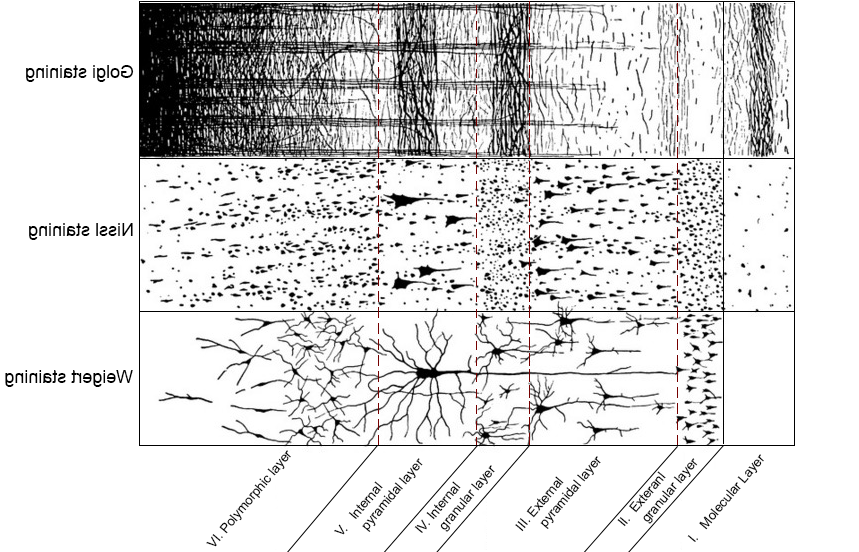
\includegraphics[width=0.8\textwidth, clip=true]{./Chapters/01_Introduction/Images/Layers}
	\caption{\cite{Brodman1909} }
	\label{fig:layers}
\end{figure}
In principle, ascending (feedforward, sensory, e.g. `I \emph{see} an apple') and descending connections (feedback, prediction, e.g. `I \emph{imagine seeing} an apple') are distinguished \cite{Rockland1979} and can be related to hierarchical ranks of processing \cite{Barone2000}. For a given node in the cortical hierarchy, it receives feedforward input that targets layer 4 and to a lesser extent layer 5 \cite{Constantinople2013} and they predominantly originate from supragranular layers (see Figure~\ref{fig:layerprocessing}). On the other hand, feedback connections from higher areas terminate primarily in layers 1 and 5, but avoid layer 4 \cite{Anderson2009}. The differential contribution is not well established \cite{Shipp2013}. This `canonical microcircuit' describes the excitatory relay of information within the cortex. While the specifics of the performed computations are largely unknown, in general, the two types of information can be somewhat speculatively linked to the predictive coding framework \cite{Friston2010}. This framework states that at the fundamental level, the brain continuously receives predictions from higher regions (feedback signal) and compares it to \emph{prediction error} from lower regions (feedforward signal). Based on this comparison, it makes new predictions and prediction errors and thus continues this in a never ending recurrent process of updating knowledge based on new information. With its link to the predictive coding, it can provide a more mechanistic understanding of the computations in the brain \cite{Shipp2016}.
\begin{figure}[!ht]
	\centering
	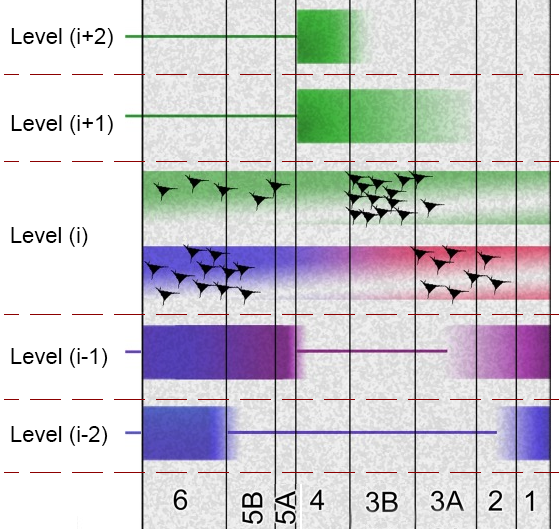
\includegraphics[width=0.5\textwidth, clip=true]{./Chapters/01_Introduction/Images/LaminarProcessing}
	\caption{Layer specific processing, adapted from Ship et al. (2013)\cite{Shipp2013}. From region $i$, there are feed forward connections (green) primarily targeting the middle layers in region higher in the cortical hierarchy ($i+1, i+2, \ell$). Feedback connections (blue, purple) target top and deep layers in lower regions in the hierarchy ($i-1, i-2, \ell$).}
	\label{fig:layerprocessing}
\end{figure}

The layers can be used to learn about information processing within a single region, but neurons also form connections with more distant regions, affording us the potential means to investigate laminar specific,  cross-regional communication. Tracer studies reveal large networks of regions via feedforward and feedback connections \cite{Felleman1991}, see Figure~\ref{fig:felleman}. Tracers heavily rely on (post mortem) structural connectivity, so even though the connections themselves can be mapped out, the strength and nature of connections remains unclear. This is why in vivo investigation of the cortical layers could add new information to the workings of directional and causal communication during task performance. Current work into interregional causal inference in the brain primarily relies on characteristics of haemodynamic consequences of brain interaction in Dynamic Causal Modelling (DCM) \cite{Friston2009} or timing differences in signals with Granger Causality \cite{Aalen2007} that can further be used to establish cortical hierarchies \cite{Michalareas2016}. The cortical layers may provide the complementary information of interregional feedforward and feedback communication in living subjects and could tell more about the crosstalk between regions at the network level.
\begin{figure}[!ht]
	\centering
	\includegraphics[width=0.6\textwidth, clip=true]{./Chapters/01_Introduction/Images/Felleman}
	\caption{Picture adapted from Felleman \& Van Essen (1991) \cite{Felleman1991}. A graphical depiction of cortical regions with structural connections as obtained by post-mortem tracer studies. This is also a rudimentary reflection of hierarchical processing in the brain. As these connections originate from and target specific layers, it would be interesting to see if similarities can be found in the layer specific fMRI signal. This could allow for making hierarchical statements about neuronal processes based on fMRI data.}
	\label{fig:felleman}
\end{figure}

Across cortical regions and across species, the layered structure of the cortex is largely conserved. It is therefore likely that many of the computational underpinnings translate from one brain region to the next \cite{Buonomano1998}. Thus, better understanding of layer specific processing in specific regions and during specific tasks could teach us more general principles of the brain. One can imagine that for some perceptual tasks, feedforward drive may dominate the computation, for example when a lot of sensory input is involved. Alternatively, when strong predictions, expectations, or imagination is involved, feedback will likely play a larger role. Linking the basic feedforward and feedback information pathways to conceptual level cognitive domains such as language, memory or emotion is a difficult task for the future, and to get a better mechanistic understanding of these evolutionary achievements, it is important to learn more about the laminar processing.

There is a variety of cognitive function in which layer specific dissociation could already be an interesting tool, as there are clear predictions with respect to feedback and feedforward drive \cite{Lawrence2017}. For example in the area of visual attention, prediction, or saliency, it could be interesting to compare and contrast the different types of hypothesised feedback drive against visual feedforward drive. It may also be used in clinical applications, as some mental disorders are expected to have abnormalities in directional communication between brain regions. Hallucinations and delusions are strongly linked to abnormal perception and are hypothesised to have different predictive coding mechanisms \cite{Fletcher2008}. This may well be reflected in neurophysiological traces of the cortical layers. Other interesting similarities with the brain are found in the emerging field of deep learning networks. Convolutional layers of the networks have been correlated to the visual hierarchy of the brain \cite{Guclu2015}, and it would be interesting to look for similarities at an even deeper level. Given that deep learning networks work with feedback and feedforward propagation of signals, if these features could be related to the cortical layers as well.

So signals from the cortical layers in a brain region may contain information about the nature of computations and about communication with other regions. Investigating this during task performance could open doors to new types of information and shed light on a multitude of cognitive processes. However, the greatest barrier is that the layers (and neuronal communication in general) are not easily measured. The most realistic current measurement technique is functional Magnetic Resonance Imaging, for its high spatial resolution and non-invasiveness. Unfortunately, fMRI does not measure neuronal firing directly, but only picks up changes in blood oxygenation that occur as a result of neuronal firing. We will therefore first need to gain a better understanding of what type of information it is that fMRI gives us.

\section*{MRI}
The basis of magnetic resonance imaging (MRI) is the phenomenon of nuclear magnetic resonance (NMR). In principle, this describes magnetic behaviour of protons and neutrons in terms of their \emph{quantum spin}: a preferred axis of rotation of an elementary particle. Normally, each spin has a random orientation of the axis of rotation. In the presence of a magnetic field, however, the spins will start precessing around the axis of the main magnetic field. The speed of rotation (angular frequency) will be directly proportional to the magnitude of the field, the Larmor frequency. In 1946, Felix Bloch and Edward Purcell (independently) performed the first experiments in which they manipulated the spins with radio frequency (RF) pulses, for which they later received a Nobel prize. Bloch described the nuclear magnetisation of a material as a function of its relaxation times $T_1$ and $T_2$ \cite{Bloch1946}. The $T_1$ value describes the time it takes for spins in a certain material to go back to their rest position after they have been excited by an RF pulse for the longitudinal magnetisation (aligned with the magnetic field). The $T_2$ value describes the time in which the transverse magnetisation (perpendicular to the magnetic field) loses the phase coherence between spins. Further development of the measurement technique allowed for a description of these properties as a function of two-dimensional space, provided by Paul C. Lauterbur in 1973 \cite{Lauterbur1973}, for which he received a Nobel prize, thirty years later. Initially, this was a much alike the tomographic back projections that form the basis of Computed Tomography (CT). This description formed the basis gradient echo imaging, where an applied magnetic field (gradient) (additional to the main magnetic field) gives rise to a signal from which an image can be reconstructed. A later description was a formalism in which the spatial frequencies of an image, $k$-space, is described as an integral of the gradient \cite{Twieg1983,Ljunggren1983}:
\begin{equation}
\vec{k}(t)=\gamma \int_{0}^{t}\vec{G}(t')dt'
\end{equation}
This is still the basis of current MR imaging. The equation represents the mapping of spatial frequencies in an image as a function of the applied gradient over time. The original simple graphical representation is shown in Figure~\ref{fig:kspace}. If the gradients are applied such that a large part of $k$-space is (homogeneously) covered, the spatial frequencies are accurately sampled. The $k$-space signal is the Fourier transform of the spin density distribution $\rho (\vec{r})$,
\begin{equation}
S(t)=\hat{\rho}(\vec{k}(t))=\int\rho(\vec{r})e^{i \vec{k}(t) \cdot \vec{r}}d\vec{r},
\end{equation}
such that the $k$-space can easily be transformed into an image of the spin density.
\begin{figure}[!ht]
	\centering
	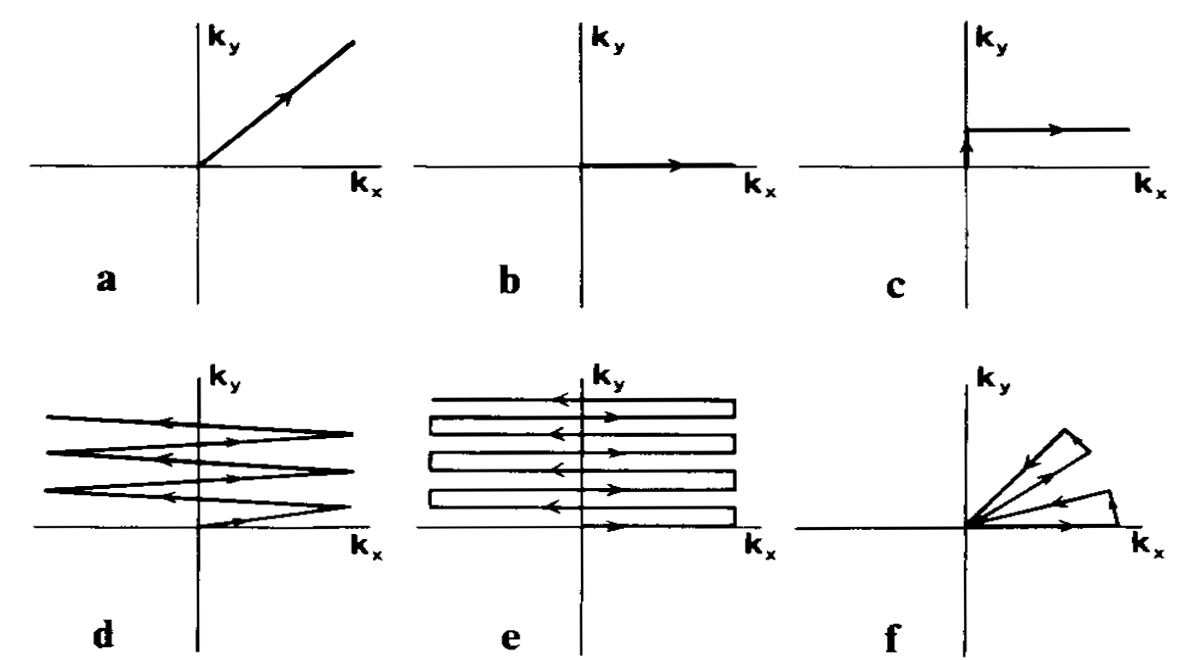
\includegraphics[width=0.6\textwidth, clip=true]{./Chapters/01_Introduction/Images/Kspace}
	\caption{ \cite{Ljunggren1983}. }
	\label{fig:kspace}
\end{figure}

The aforementioned $T_1$ and $T_2$ mechanisms occur as random processes of spins getting back to a rest equilibrium. There is an additional mechanism, $T_2^*$, in which the dephasing of the spins is not random but predictable, and thus reversible. After an RF pulse, spins start out by pointing in the same direction, but then fan out and start to dephase in clockwise or counter clockwise direction. Hence, the spins will cancel each other out, such that the signal decays much faster than $T_2$, but instead with $T_2^*$. However, their direction can be reversed (by a 180\textdegree RF pulse), such that they start to converge until they point in the same direction again to form a \emph{spin echo}. As a result gradient echo images are $T_2^*$-weighted and spin echo images are $T_2$-weigthed. In general, there is a variety of different acquisition sequences that all target different magnetic properties of the scanned object.

A different contrast is that of Arterial Spin Labelling (ASL) \cite{Williams1992,Detre1994}. In this technique, arterial blood is first `labelled' by means of a 180\textdegree pulse (Figure~\ref{fig:asl}). The labelled blood has different magnetisation and travels downstream where, after an inversion time, the spins in a small area are again inverted by a 180\textdegree pulse. This latter is repeated in a scenario without the initial labelling. The difference in signal must be due to inflow of blood after the original arterial spin labelling. This way, ASL is sensitive to cerebral blood flow (CBF) and can produce perfusion images of the brain \cite{Petcharunpaisan2010}.
\begin{figure}[!ht]
	\centering
	\includegraphics[width=0.6\textwidth, clip=true]{./Chapters/01_Introduction/Images/Asl}
	\caption{}
	\label{fig:asl}
\end{figure}

Next to cerebral blood \emph{flow}, one can also look at cerebral blood \emph{volume}. Blood vessels may dilate and contract as a function of the activity of a brain region. This can be measured with Vascular Space Occupancy (VASO) \cite{Lu2003}. VASO makes use of the fact that the $T_1$ values of arterial and venous blood are very close together and both a lot shorter than the $T_1$ of tissue. By inverting all signal and measuring at an inversion time where the blood signal goes through zero, the only signal that is left has to come from tissue. Effectively, the remaining signal represents the contribution of tissue in a voxel. On neuronal activation, blood vessels expand and increase in voxel contribution, which decreases the tissue contribution and lowers the signal. Thus, the VASO signal goes down on activation and looks like a negative BOLD signal.

\section*{Contrast Mechanisms}
So MRI scanners can be used to obtain a variety of types of information, but is any of it relevant to the study of cortical layers? At the core, all contrasts are results of changes in magnetic properties. All materials have a magnetic \emph{susceptibility}, the extent to which it becomes magnetised by an external magnetic field. If the material resists the magnetic field (i.e. negative susceptibility) it is diamagnetic, and if it assists the field (i.e. positive susceptibility) it is paramagnetic. Certain metals (e.g. iron, nickel, cobalt) have very high susceptibility and are called ferromagnetic. These are the materials that are commonly attracted by standard refrigerator magnets. Red blood cells contain haemoglobin that is paramagnetic when it does not carry oxygen (deoxyhaemoglobin) because of the high spin state of the iron atom \cite{Pauling1936}. The change in magnetic susceptibility of red blood cells when they are oxygen rich or oxygen poor is called the Blood Oxygenation Level Dependant Signal, the BOLD signal \cite{Ogawa1990}. So while neuronal firing does not change magnetic properties directly, synaptic activity indirectly causes changes in blood flow that may be picked up with an MRI scanner \cite{Logothetis2006}. It is of note that large parts of the biological mechanisms behind the neurovascular relationship are still disputed; most importantly, the extent to which the BOLD response reflects laminar specific activation is largely unknown.

Fundamentally, the BOLD signal arises as a consequence of magnetic field perturbations arising from desoxyhaemoglobin molecules \cite{Norris2006}. These changes extend beyond the blood vessel into the tissue and drop off as a function of field strength, the orientation of the vessel, and the vessel diameter as well as the concentration of deoxyhaemoglobin. From the time that the molecules are excited until the time of the echo, molecules in the tissue move around the vasculature. If the trajectory of a molecule in this time is small compared to the vessel size (and hence compared to the drop-off), there is little change in its surrounding magnetic field and the effect is reversible, a static effect. If on the other hand the molecule's trajectory is large, its surrounding magnetic field changes more drastically and unpredictably, such that the effect is irreversible and dynamic. These two contrast mechanisms are the static and dynamic extravascular effect. The magnetic field perturbations around the vessels scale linearly with field strength, so the trajectory of a molecule relative to the perturbations is much greater at 7 Tesla than at 1.5 Tesla. Thus, the relative contribution of the dynamic extravascular effect increases with field strength. Specifically, the static effect increases linearly with field strength and the dynamic effect increases quadratically. The remaining static effect at 7 Tesla is thus very specific, but detecting it requires high sensitivity \cite{Panchuelo2014}.

An additional source of BOLD contrast is the intravascular effect. The magnetic field inside the vessel is slightly different from the surrounding tissue because of the amount of desoxyhaemoglobin. As a result, the signal will start to dephase with respect to the extravascular signal. This can be reversed because it is constant over time and is called the static intravascular effect. The last contrast mechanism that contributes to the BOLD signal is disputed in origin. This is irreversible (dynamic) intravascular dephasing and has to do with the random movement of water molecules within red blood cells. It is either due to these water molecules interacting with the deoxyhaemoglobin, or with the diffusion in and out of the cells, but no experiment to date has been able to tease the two mechanisms apart.

The 180\textdegree pulses in spin echo reverse all static effects, as the dephasing is flipped to return to its initial position. Therefore, spin echo is only susceptible to the ($T_2$-weighted) dynamic contrast mechanisms and less sensitive than gradient echo to which all four mechanism contribute. But by losing the static intravascular effect, the large contribution of the draining veins on top of the cortex is invisible to spin echo, increasing its specificity. Towards higher field, the proportion of extravascular dynamic contrast increases with respect to the intravascular dynamic contrast \cite{Norris2002,Jochimsen2004,Norris2006}. This makes spin echo even more specific at higher field strength. Unfortunately, it is harder to run spin echo sequences at higher fields, as the number of 180\textdegree pulses increases the specific absorption rate to the extent that the brain heats up more than is allowed by current safety limits. So both spin echo and gradient echo have advantages and disadvantages. A range of laminar profiles has been found using spin echo (e.g. \cite{Zhao2004,Harel2006,Goense2006}) or gradient echo (e.g. \cite{Polimeni2010,DeMartino2013,Chen2013}). Also a combination of both has been tried, GRadient A Spin Echo (GRASE) \cite{Olman2012,DeMartino2013}.

Given the four BOLD contrast mechanisms, it is still an outstanding question in what proportions they contribute in measurements. This may even vary at the laminar level, as the deoxyhaemoglobin from deeper layers flows upward to the top layers. The relative contributions of the contrast mechanisms in combination with the blood flow effect has been modelled for both spin echo and gradient echo and suggest that most of the signal produced in a layer is also visible in that layer \cite{Markuerkiaga2016,Uludag2017}. For spin echo the flow effect is minimal, while gradient echo has a tail that extends to more superficial layers, but at a gain of sensitivity. 

Figure~\ref{fig:microvasulature} shows the microvasculature of a small piece of visual cortex in a macaque. In red, the arterioles, small blood vessels that dive from the top of the cortex (the pial surface) downward to supply the whole grey matter with blood. The smallest vessels, the capillaries, relay the oxygen to the neurons in all cortical layers, such that deoxygenated haemoglobin is drained away by the veins (blue). The veins on top of the cortex can be an order of magnitude larger than the cortical veins, and accumulate and carry off the deoxygenated blood. This might make one appreciate the difficulty of extracting laminar specific signals with large signals of non-interest in the direct neighbourhood.
\begin{figure}[!ht]
	\centering
	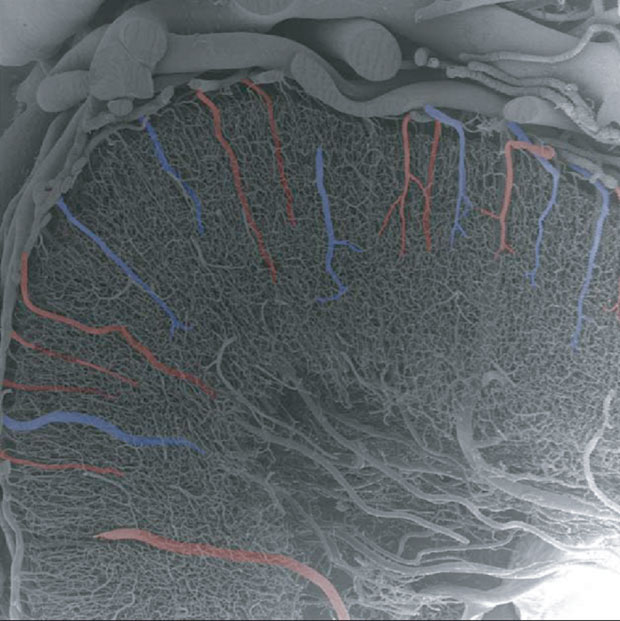
\includegraphics[width=0.9\textwidth, clip=true]{./Chapters/01_Introduction/Images/Microvasculature}
	\caption{The microvasculature of the visual cortex of a macaque \cite{Weber2008}. }
	\label{fig:microvasulature}
\end{figure}

The level of measured blood oxygenation depends on several factors. On activation, more blood starts flowing (higher cerebral blood flow, CBF), vessels start dilating (more cerebral blood volume, CBV) and the consumption of oxygen increases (higher cerebral metabolic rate of oxygen, CMRO$_{2}$). These quantitative measures can be related to one another, save some free parameters that need to be empirically determined \cite{Davis1997}. However, the proposed equations hold for the cortical column in its entirety, but do not take into account potential layer specific differences. So while we cannot measure neuronal activation with MRI, the closest we can get is the traces in magnetic properties in the vasculature through BOLD, CBV, CBF, and CMRO$_{2}$. The extent to which these quantities vary as spatially specific as the level of the cortical layers is an outstanding question, however, and needs to empiraclly tested. Indeed, there are techniques to measure them, $T_2^*$-weighted imaging for BOLD \cite{Norris2006}, VASO for CBV \cite{Huber2018}, arterial spin labelling for CBV \cite{Grade2015}, and calibrated BOLD for CMRO$_{2}$ \cite{Blockley2013}. All vary in terms of sensitivity, specificity, and attainable resolution (spatial as well as temporal). The spatial resolution in combination with the type of experiment that is required for CBF and CMRO$_2$ measurements makes them poor candidates for human in vivo fMRI. It is mainly BOLD and CBV that have shown promising layer specific differences in animal experiments \cite{Lu2004,Zhao2006,Jin2008,Goense2012}. The main benefits of VASO compared to BOLD are its quantifiability \cite{Lu2003} and local specificity \cite{Jin2006}, whereas BOLD has higher sensitivity and speed \cite{Huber2018}.

\section*{Acquisition}
We have seen that MRI can be used to measure different magnetic properties, potentially in combination with physical and physiological properties of the brain. For our purposes, we are interested mainly in the properties of the BOLD response, which we use to rapidly create images of the brain. Every few seconds, an image is acquired that is a reflection of the BOLD response at that moment. We would like to have as many images as possible as we aim to measure real-time responses to our experiments. As a result, we may have to make compromises in the spatial resolution, signal to noise ratio, or contrast to noise ratio. Functional ($T_2^*$-weigthed) images are optimal for measuring BOLD activity, but do not show a particularly clear difference between the white matter and the grey matter (see Figure~\ref{fig:mybrain}). For accurately distinguishing the cortical layers, another image is required with better anatomical contrast. For this, a structural (or anatomical) scan is used. It cannot be acquired in several seconds, as the functional scan, and instead takes several minutes. A structural scan is $T_1$-weighted and shows high anatomical contrast because the $T_1$-value of the myelinated white matter is shorter than the $T_1$-value of grey matter \cite{Wansapura1999}. It is often sufficient to compute a cortical reconstruction, a three-dimensional representation of the cortical surface. A cortical reconstruction can be a useful way of looking at the brain as a geometrical shape and can facilitate a variety of subsequent analyses.
\begin{figure}[!ht]
	\centering
	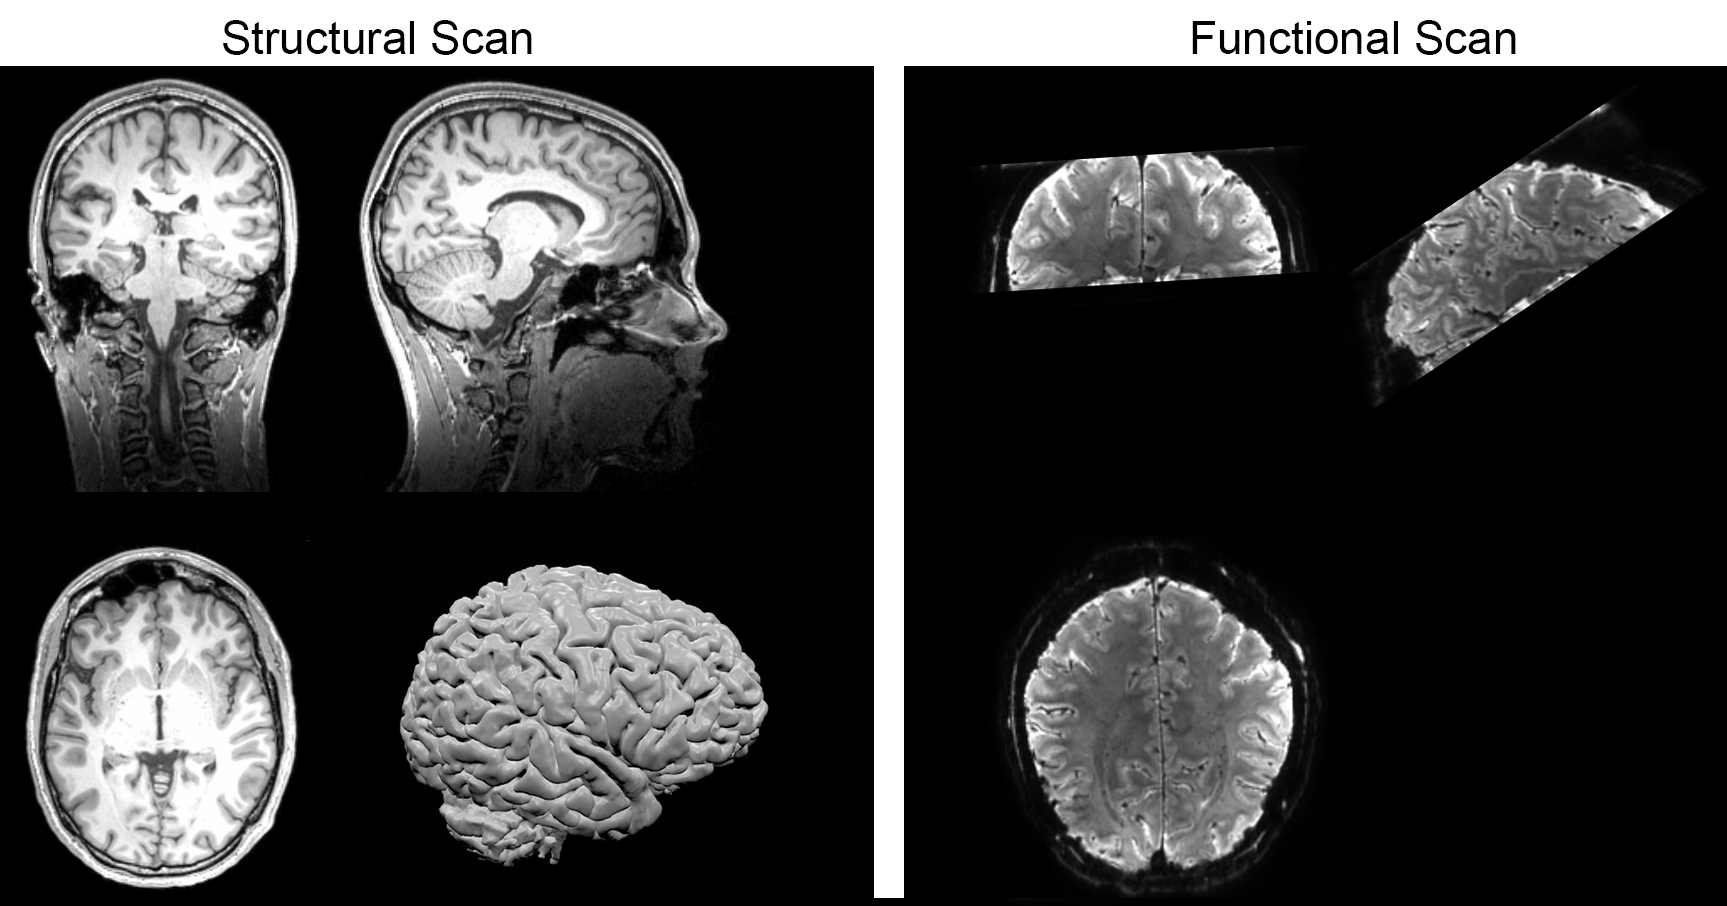
\includegraphics[width=0.99\textwidth, clip=true]{./Chapters/01_Introduction/Images/MyBrain}
	\caption{An example of a structural and functional brain scan. On the left, the structural scan has high anatomical contrast and sharp differences between the white matter and grey matter. The contrast is sharp enough to make a three dimensional reconstruction of the brain (lower right corner). On the right, a functional image is shown. The anatomical contrast is much weaker, but it can be acquired quickly and the contrast is susceptible to slight changes in blood deoxyhemoglobin, related to oxygen consumption on neuronal activation.}
	\label{fig:mybrain}
\end{figure}

Much research has been done to retrieve new types of information with MRI. Complementary to this, improving the speed of the acquisition has always been an important point of development. There is a variety of ways in which this can be done. Acceleration techniques can make use of mathematical properties of the acquired signal (Hermitian symmetry of the $k$-space), in order to acquire only a part of the $k$-space in partial Fourier acquisitions \cite{Feinberg1986}. Alternatively, information can be added to the reconstruction equations by adding in information about the sensitivity of receiver coils. Techniques like GRAPPA, SENSE, and CAIPIRINHA use this type of information which can make the acquisition several times faster \cite{Setsompop2016}. In general, MRI data contains several forms of spatiotemproal redundancy that can be exploited to speed up the acquisition \cite{Tsao2012}. Using these techniques is essential to increase the spatial resolution, temporal resolution, or the signal to noise ratio per volume.

The acquisition of anatomical scans is relatively straightforward as there is no pressure to acquire a volume every several seconds. One can rely on standard acquisition protocols for MPRAGE sequences \cite{Mugler1990} or a version that is less susceptible to intensity biases but that takes longer to acquire, the MP2RAGE \cite{Marques2010}. For functional images, there are more constraints and parameters to consider, of which we will here discuss the difference between 2D and 3D acquisitions. A three-dimensional MRI volumes can be acquired in several ways. In a 2D acquisition, a stack of slices is sequentially acquired and put on top of each other. This requires excitation of a single slice at the time, and the two-dimensional encoding of each plane. For each plane, the $k$-space (all spatial frequencies) is sampled and converted to an image by means of a Fourier transform. This makes for a smooth planar image, but as the stack of images is scanned sequentially, the vertical transition ($z$-direction) may be less smooth. Every movement of the brain during the acquisition will result in images not precisely landing on top of each other such that images may show a `staircase artifact' in the vertical direction. The higher the resolution, the more pronounced this staircase artifact will be. In addition, towards higher resolution the two-dimensional excited slabs need to get smaller, which requires a sharper slice profile. This in turn requires longer pulses that easily cause higher specific absorption rates and may cause peripheral nerve stimulation. Many of these factors can be circumvented with a 3D acquisition \cite{Poser2010}. Instead of a plane-by-plane excitation and read-out, the entire volume is excited \cite{Song1994} to fill a three-dimensional $k$-space. The image can then be reconstructed by a single three-dimensional Fourier transform instead of a series two-dimensional Fourier transforms. This way, transitions between slices are smoother, which is important for cortical layering. As a downside, any movement during the acquisition will cause noise (blurring) in the entire image so 3D imaging is more vulnerable to physiological effects. However, this is generally outweighed by the shorter volume TR that can more easily be achieved by acceleration techniques \cite{Poser2010}. Because there is no limitation of slice-by slice acquisition in the $z$-direction, this dimension can be used for parallel imaging. At high spatial resolution, 3D imaging is faster and has a higher sensitivity.

Choosing a sequence requires carefully balancing the advantages and disadvantages against each other. We here chose to use gradient echo with a 3D EPI acquisition to investigate the laminar BOLD signal for its higher sensitivity and at a field strength of 7 Tesla for high specificity. The potential downside of this is the susceptibility to the larger veins on top of the cortex that might obscure smaller effects \cite{Barth2007}.

\section*{FMRI analysis}
After covering the fundamentals of measurement techniques, it is clear what types of information may be expected to be present in the data. Getting out the relevant information, however, is at least as complicated. The brain is a highly convoluted structure that we are trying to describe and visualise by means of cubic voxel rasters. The first problem we encounter is a geometrical one: how do we attach a brain location to voxels in space? This can be done by making a \emph{cortical reconstruction} on a high resolution brain scan \cite{Dale1999,Bazin2012} with a very clear contrast between the white matter and grey matter as seen in Figure~\ref{fig:mybrain}. The distinction between white and grey matter is clear enough to draw a three-dimensional boundary on both side of the grey matter: on the white matter boundary and on the pial surface, the separation between the grey matter and the cerebrospinal fluid (CSF).

The cortical reconstruction is very informative about the shape of the brain and potentially also about the layers: One could imagine different layers to be described as intermediate surfaces between both outer boundaries of which the locations can be used to then sample the cortical layers \cite{Koopmans2011,Polimeni2010,DeMartino2013}. This description allows for all sorts of surface based calculations \cite{Fischl2000,Bazin2012} and for example allows us to take into account a more naturalistic flow of the cortical layers \cite{Bok1929,Waehnert2014}. Along the many curves of the cortex, cytoarchitectonic layers approximately conserve volume in a given cortical column. Taking this into account can provide a clear advantage in high resolution laminar analysis.

The cortical reconstruction can be made on a dedicated high resolution high contrast scan, but this does not yet give functional information. First, the cortical surfaces need to be `coregistered' with the functional data and brought into the same analysis space. Unfortunately, this is made considerably more difficult by two main factors. First, the contrast and resolution of standard gradient echo functional data is poor, so there is not a lot of information on which to base a good coregistration. Secondly, when `echo planar imaging' (EPI) is used, a fast acquisition scheme to collect data, the data will to some extent be geometrically distorted. The reason is that the scanner magnetic field is not everywhere exactly equal. When we talk about a scanner with a field strength of 7 Tesla, it means there should be a stable static magnetic field of that strength in the centre of the scanner. However, because the presence of a human body perturbs the field, it is not as homogeneous as one might desire. Small perturbations can be corrected by \emph{shimming}, applying an additional magnetic field to compensate for the inhomogeneities. However, this is not accurate enough to correct all deviations and the inhomogeneities need not even be constant over time. As mentioned before, MRI is based on spins precessing at a frequency that is proportional to the field strength.
If the field is slightly higher or lower, the spins in that area precess slightly faster or slower. It was noted that MRI measures spatial frequencies of an image, assuming a constant magnetic field. So one could imagine that as a direct result of the Fourier shift theorem, spins that precess faster or slower are instead displaced in the resulting image. Since the displacement is field strength dependent, distortions are more pronounced at higher fields. They can easily be of the order of several millimetres, which comes down to a shift of the size of the entire cortex. So extreme care must be taken in aligning scans properly and thoroughly checking the correctness of the cortical surface in the regions that one wants to analyse.

%The distortions are only present in the phase encoding direction because
% as a function of BW per pixel and field strength \cite{Jezzard1995,Schmitt1998}
%%I think you can improve this explanation, for example why is distortion only along phase-encoding axis.

There is a wide variety of other potential sources of noise that can contaminate the (laminar) signal. Participants in a study will move several millimetres, breathe and have a heartbeat that is clearly visible in the signal, people may have lapses in their attention, may even fall asleep, et cetera. Many operations are performed on the data to remove as many sources of noise as possible and this creates long analysis pipelines. This makes the process of doing fMRI analysis difficult at the conceptual level, and may also create a logistical nightmare: different software packages, programming languages, data types, data representations, and different styles of programming. As a result, it is understandable that the reproducibility of fMRI results can be low \cite{Nosek2015,Gorgolewski2016a}. We here took care to build and use all tools as reproducibly as possible and to provide all data openly, accompanied with the scripts to generate the results.

\section{Laminar Analysis in Human FMRI}
A lot of information about the computations in the brain may lie in better understanding the cortical layers. Invasive electrophysiological recordings indeed find relevant laminar differentiation in macaques \cite{Buffalo2011,Maier2010,Maier2011,VanKerkoerle2017}, and while the exact origins of the BOLD signal are still unknown, there is strong evidence that the BOLD signal has a laminar footprint \cite{Goense2006}. This is confirmed by Yu et al. \cite{Yu2014}, where they show clear layer specificity in the onset of the BOLD response, but no prolonged laminar differentiation that could be picked up with the temporal resolution of conventional human fMRI. While it is known which layers are initially targeted by feedback and feedforward signals, little is known about their further processing. There is evidence that excitatory neurons may quickly redistribute input from the thalamus by means of their local axonal collaterals \cite{Guy2017,ReyesPuerta2015}. As a result, cortical activity may nearly instantaneously spread over several layers and columns, to the detriment of laminar specificity of the BOLD signal.

But there is also a substantial body of work that claims to have found hypothesised laminar differentiation in humans \cite{Maass2014,Muckli2015,Kok2016,Huber2017}. Unfortunately, all of them use different methods for largely the same type of analysis. To date no published replications exist of layer specific human in vivo studies that could reinforce these findings. With the variations in analysis, many uncertainties in the data, and the small size of the potential effect, it is clear that any potential effect can only be picked up with powerful methods that address as many sources of noise as possible. In this thesis, we made a robust and reusable analysis pipeline in which we solved key issues in laminar analysis and envision laminar specific investigations a more routine type of study.


